La complexit\'e d'une suite de symboles
peut se mesurer par la taille minimum d'un code
permettant de reconstruire cette suite.
La th\'eorie de l'information de Shannon montre que le nombre
de bit moyen pour coder chaque symbole d\'epend de l'entropie
du processus al\'eatoire sous-jacent.
Pour coder des suites de nombre r\'eels, il est necessaire
de les approximer avec une quantification avant d'effectuer
un codage entropique.
L'optimisation de cette quantification est \'etudi\'ee.
Ces r\'esultats donnent les bases math\'ematiques
et algorithmiques permettant de
comprimer des signaux audios ou des images.

\section{Complexit\'e et Entropie}

La th\'eorie de l'information d\'efinie la complexit\'e d'une
s\'erie num\'erique en \'evaluant la taille des codes permettant
de reproduire cette s\'erie. Les fondations de cette th\'eorie
sont mises en place par Shannon en 1948, qui mod\'elise
des s\'eries num\'eriques comme des r\'ealisations d'un processus
al\'eatoire. Il d\'emontre alors
l'existence d'une complexit\'e intrins\`eque associ\'ee \`a tout
processus al\'eatoire, qu'il appelle {\it entropie}.
En 1965, Kolmogorov introduit une d\'efinition plus
g\'en\'erale de la complexit\'e d'une s\'erie num\'erique,
comme \'etant la longueur minimum du programme binaire
permettant de reproduire cette s\'erie avec un ordinateur.
Le mod\`ele d'ordinateur est une machine de Turing ayant un
nombre fini d'\'etats.
Cette d\'efinition n'a pas recours \`a un mod\`ele probabiliste
mais est plus d\'elicate \`a manipuler math\'ematiquement.
Nous suivront donc ici l'approche de Shannon qui donne des
r\'esultats suffisament pr\'ecis pour la plupart des
probl\`emes de traitement du signal.

\subsection{Suites typiques}

Consid\'erons des suites de symboles de taille $n$ prenant leurs
valeurs dans un alphabet $A = \{a_k \}_{1 \leq k \leq K}$
de taille $K$.
L'approche probabiliste de Shannon mod\'elise
ces s\'equences de symboles comme \'etant les valeurs prises
par des variables al\'eatoires $X_1\, X_2\,\dots\, X_n$.
Pour simplifier l'analyse, nous nous placerons dans le cas le
plus simple o\`u les $X_i$ sont des variables al\'eatoires
ind\'ependantes et de m\^eme loi. On note
\[
p(a_k) = \PP \{ X_i = a_k \} .
\]
Comme les variables $X_i$ sont ind\'ependantes, la
probabilit\'e d'une suite de valeurs est:
\[
p(x_1,\, \dots\,, x_n) = \PP \{X_1 = x_1 ,\, \dots\, , X_n = x_n \} =
\prod_{k=1}^n \PP \{X_k = x_k \} = \prod_{k=1}^n p(x_k) .
\]
On peut d\'efinir $p(X_1 ,\, ..\, X_n) = \prod_{k=1}^n p(X_k)$
qui est une variable al\'eatoire donnant la probabilit\'e
d'une suite de valeurs tir\'ee au hasard.
Le th\'eor\`eme suivant montre que pour $n$ fix\'e
et suffisament grand, alors pour la plupart des
tirages, cette probabilit\'e est presque constante et
\'egale \`a l'entropie
\[
H = - \sum_{k=1}^K p(a_k)\, \log_2 p(a_k) = - E\{ \log_2 p(X_i)\} .
\]
L'entropie $H$ peut s'interpr\'eter comme
l'incertitude moyenne sur les valeurs
que prennent les variables al\'eatoire $X_i$.
On peut v\'erifier que
\[
0 \leq H \leq \log_2 K .
\]
L'entropie est maximum, $H = \log_2 K$, si
$p(a_k) = \frac 1 K$ pour $1 \leq k \leq K$.
Il y a en effet une incertitude maximum sur les valeurs prises
par $X_i$.
L'entropie est minimum, $H = 0$, si l'un des symboles $a_k$
a une probabilit\'e $1$.
On conna\^{\i}t alors \`a l'avance la valeur de $X_i$.

\begin{theorem}
\label{EquiTh}
Si les $X_i$ sont des variables al\'eatoires ind\'ependantes
et de m\^eme probabilit\'e $p(x)$ alors
\[
-\frac 1 n \log_2 p(X_1, \dots,X_n)~~\mbox{tend vers $H$ avec
une probabilit\'e $1$}
\]
lorsque $n$ tend vers $+\infty$.
\end{theorem}
\begin{proof}
On calcule
\[
- \frac 1 n \log_2 p(X_1,\, \dots ,, X_n) = - \frac 1 n \sum_{i=1}^n
\log_2 p(X_i)~.
\]
Comme les $X_i$ sont ind\'ependants, les $\log_2 p(X_i)$ sont aussi
des variables al\'eatoires ind\'ependentes.
En appliquant la loi forte des grands nombres 
on d\'emontre que
$- \frac 1 n \sum_{i=1}^n \log_2 p(X_i)$ tend
vers $- E\{ \log p(X_i)\} = H$ lorsque $n$ tend vers $+\infty$,
avec probabilit\'e 1.
\end{proof}

Bien qu'a priori $X_1,\,\dots\,,X_n$ puisse prendre des
valeurs quelconques dans l'ensemble $A^n$ des vecteurs de
symboles de taille $n$, ce th\'eor\`eme permet de montrer
qu'il y a une probabilit\'e presque $1$ pour que ce vecteur soit
une suite typique appartenant \`a un ensemble beaucoup plus
petit. On appelle {\it ensemble typique} $T^n_\epsilon$
relativement \`a $p(x)$ l'ensemble des suites
$(x_1,\dots,x_n) \in A^n$ telles que
\begin{equation}
\label{Typique-def}
2^{-n (H+\epsilon)} \leq p(x_1,\dots,x_n) \leq
2^{-n (H-\epsilon)} .
\end{equation}
On note $|T^n_\epsilon|$ le cardinal de $T^n_\epsilon$.
Le th\'eor\`eme suivant montre que
$|T^n_\epsilon|$
est de l'ordre de $2^{nH}$, et que toutes les
suites typiques ont une probabilit\'e presque \'egale
\`a $2^{-nH}$.

\begin{proposition} [Ensembles typiques]
\begin{enumerate}[label=(\roman*)]
\item  Si $(x_1, \dots , x_n) \in T^n_\epsilon$ alors
\begin{equation}
\label{Typique-th1}
H - \epsilon \leq - \frac 1 n \,\log_2 p(x_1, \dots , x_n)  \leq H + \epsilon .
\end{equation}
\item Lorsque $n$ est suffisamment grand
\begin{equation}
\label{Typique-th2}
\PP \{(X_1, \dots,X_n) \in T^n_\epsilon \} > 1 - \epsilon .
\end{equation}
\item  Lorsque $n$ est suffisamment grand
\begin{equation}
\label{Typique-th3}
2^{n(H - \epsilon)} \leq |T^n_\epsilon| \leq
2^{n(H + \epsilon)} .
\end{equation}
\end{enumerate}
\end{proposition}
\begin{proof}
La propri\'et\'e (\ref{Typique-th1}) est une
cons\'equence directe de la d\'efinition (\ref{Typique-def})
de $T^n_\epsilon$.

L'in\'egalit\'e (\ref{Typique-th2})
se d\'eduit du th\'eor\`eme \ref{EquiTh} qui montre
que pour tout $\epsilon>0$ et $\delta > 0$ il existe $n_0$
tel que pour tout $n \geq n_0$
\[
\PP \left\{\left|  -\frac 1 n \log_2 p(X_1, \dots , X_n) - H \right|
< \epsilon \right\} >
1 - \delta .
\]
En prenant $\delta = \epsilon$ on obtient (\ref{Typique-th2}).

On note $\vec x = (x_1 , \dots , x_n)$,
\begin{eqnarray*}
1 &=& \sum_{\vec x \in A^n} p(\vec x) \geq \sum_{\vec x \in T^n_\epsilon} p(\vec x) \\
& \geq & \sum_{\vec x \in T^n_\epsilon} 2^{-n(H +\epsilon)} =
|T^n_\epsilon|\, 2^{-n(H +\epsilon)} ,
\end{eqnarray*}
ce qui d\'emontre l'in\'egalit\'e (\ref{Typique-th3})
\`a droite.

Lorsque $n$ est suffisament grand, on a montr\'e en
(\ref{Typique-th2}) que
\begin{eqnarray*}
1 - \epsilon & < &\PP \{(X_1, \dots,X_n) \in T^n_\epsilon \} \\
& \leq & \sum_{x \in T^n_\epsilon} 2^{-n(H-\epsilon)} =
|T^n_\epsilon| \, 2^{-n(H-\epsilon)} ,
\end{eqnarray*}
ce qui d\'emontre l'in\'egalit\'e (\ref{Typique-th3})
\end{proof}

\subsection{Codage}
On peut effectuer un codage ``$\epsilon$-typique'' des
valeurs de $X_1\,\dots,X_n$ qui utilise des mots binaires plus courts
pour coder les s\'equences typiques qui sont les plus probables.
Comme il y a moins de $2^{n(H+\epsilon)}$ \'el\'ements
dans $T^n_\epsilon$, ces \'el\'ements peuvent \^etre ind\'ex\'es
par des mots binaires de $\lfloor n(H+\epsilon)\rfloor + 1$
bits, o\`u  $\lfloor x \rfloor$ est le plus grand entier inf\'erieur
\`a $x$.
Comme il y a $K^n$ \'elements dans $A$, les \'el\'ements
qui n'appartiennent pas \`a $T^n_\epsilon$ peuvent \^etre
ind\'ex\'es par des mots binaires de
$\lfloor \log_2 K \rfloor + 1$ bits. Afin de savoir si
$x \in T^n_\epsilon$ on rajoute
un $0$ au d\'ebut de son code binaire, qui est donc de longueur
$\lfloor n(H+\epsilon)\rfloor + 2$. Si $x \in T^n_\epsilon$
on rajoute un $1$ au d\'ebut de son code binaire, dont la
taille est donc $\lfloor \log_2 K \rfloor + 2$.
On note $R$ le nombre moyen de bits pour coder chaque
symbole d'une sequence $X_1, \dots , X_n$.


\begin{theorem}
Il existe $C > 0$ tel que pour tout
$\epsilon > 0$, et $n$ suffisament grand,
le nombre moyen $R$ de bits par symbole d'un
codage $\epsilon$-typique satisfait
\[
R \leq H + C\, \epsilon .
\]
\end{theorem}
\begin{proof}
On note $\vec X = (X_1, \dots , X_n )$,
$\vec x = (x_1 , \dots , x_n )$. Soit $l(x_i)$ la longueur du
mot binaire utilis\'e par un code typique pour coder $x_i$.
Le nombre total de bits pour coder $\vec x$ est
\[
l(\vec x) = \sum_{i=1}^n l(x_i)~.
\]
Le nombre moyen de bits par symbole est donc
\begin{eqnarray*}
R &=& E \{ l(\vec X)\} =
\sum_{\vec x \in A^n} l(\vec x)\, p(\vec x) =
\sum_{\vec x \in T^n_\epsilon} l(\vec x)\, p(\vec x) +
\sum_{\vec x \nin T^n_\epsilon} l(\vec x)\, p(\vec x) \\
&\leq& \PP \{\vec X \in T^n_\epsilon \}\,
\Bigl(\lfloor n(H+\epsilon)
\rfloor + 2\Bigr)
+ \PP \{\vec X \in T^n_\epsilon \}\,
\Bigl( \lfloor n \log_2 K \rfloor +
2\Bigr) \\
&\leq& n(H+\epsilon) + 2 + \epsilon ( n \log_2 K + 2) \leq
 H + C\, \epsilon
\end{eqnarray*}
avec $C = 5 + \log_2 K $ pour $n \geq 1/\epsilon$.
\end{proof}
Ce th\'eor\`eme d\'emontre que l'on peut construire un code
dont le nombre de bit moyen par symbole est arbitrairement
pr\`es de l'entropie $H$. Par ailleurs, on peut montrer
que tout code n\'ecessite un nombre moyen de bit par symbole $R \geq H$. Le paragraphe
suivant d\'emontre ce r\'esultat pour les codes par blocs.


\subsection{Codage entropique}
\label{entropy-code-sec}

Nous considerons dans un premier temps
les codes instantan\'es, qui d\'efinissent un code binaire
$w_k$ pour chaque symbole $a_k$ de l'alphabet $A$. Cela
permet de d\'ecoder symbole par symbole toute
s\'equence $x_1, \dots, x_n$.
Si $\log_2 K$ est un entier, chaque symbole
$a_k$ peut \^etre cod\'e par un mot binaire de
$\lfloor \log_2 K \rfloor + 1$ bits.
Ce code peut cependant \^etre am\'elior\'e
en utilisant des mots
binaires plus courts pour des symboles qui apparaissent plus
souvent.

Soit $l_k$ la longeur du code binaire
$w_k$ associ\'ee \`a $a_k$.
Le nombre moyen de bits n\'ecessaires pour coder les symboles
d'une suite de variables al\'eatoires $X_1 \, \dots\, X_n$ de
m\^eme probabilit\'e $p(x)$ est
\begin{equation}
\label{bit-rate}
R  = \sum_{k=1}^{K} l_k\, p(a_k) .
\end{equation}
Le but est de trouver un code instantan\'e qui soit
d\'ecodable et qui minimise $R$.\\

\subsection{Condition de pr\'efixe}
Un code instan\'e n'est pas toujours uniquement d\'ecodable.
Par exemple, le code qui associe \`a
$\{a_k\}_{1 \leq k \leq 4}$
les mots binaires
\[
\{w_1 = 0 ~,~w_2 = 10 ~,~w_3 = 110 ~,~w_4 = 101 \}
\]
n'est pas d\'ecodable de fa\c{c}on unique.
La suite $1010$ peut soit correspondre
\`a $w_2~w_2$ ou \`a $w_4~ w_1$.
La condition de pr\'efixe impose qu'aucun mot binaire n'est le
d\'ebut d'un autre mot binaire.
Cette condition est clairement n\'ecessaire et
suffisante pour garantir que
toute suite de mots binaires se d\'ecode de fa\c con unique.
Dans l'exemple pr\'ec\'edent,
$w_2$ est le pr\'efixe de $w_4$.
Le code suivant
\[
\{w_1 = 0 ~,~w_2 = 10 ~,~w_3 = 110 ~,~w_4 = 111 \}
\]
satisfait la condition de pr\'efixe.


\begin{figure}[bhtp]
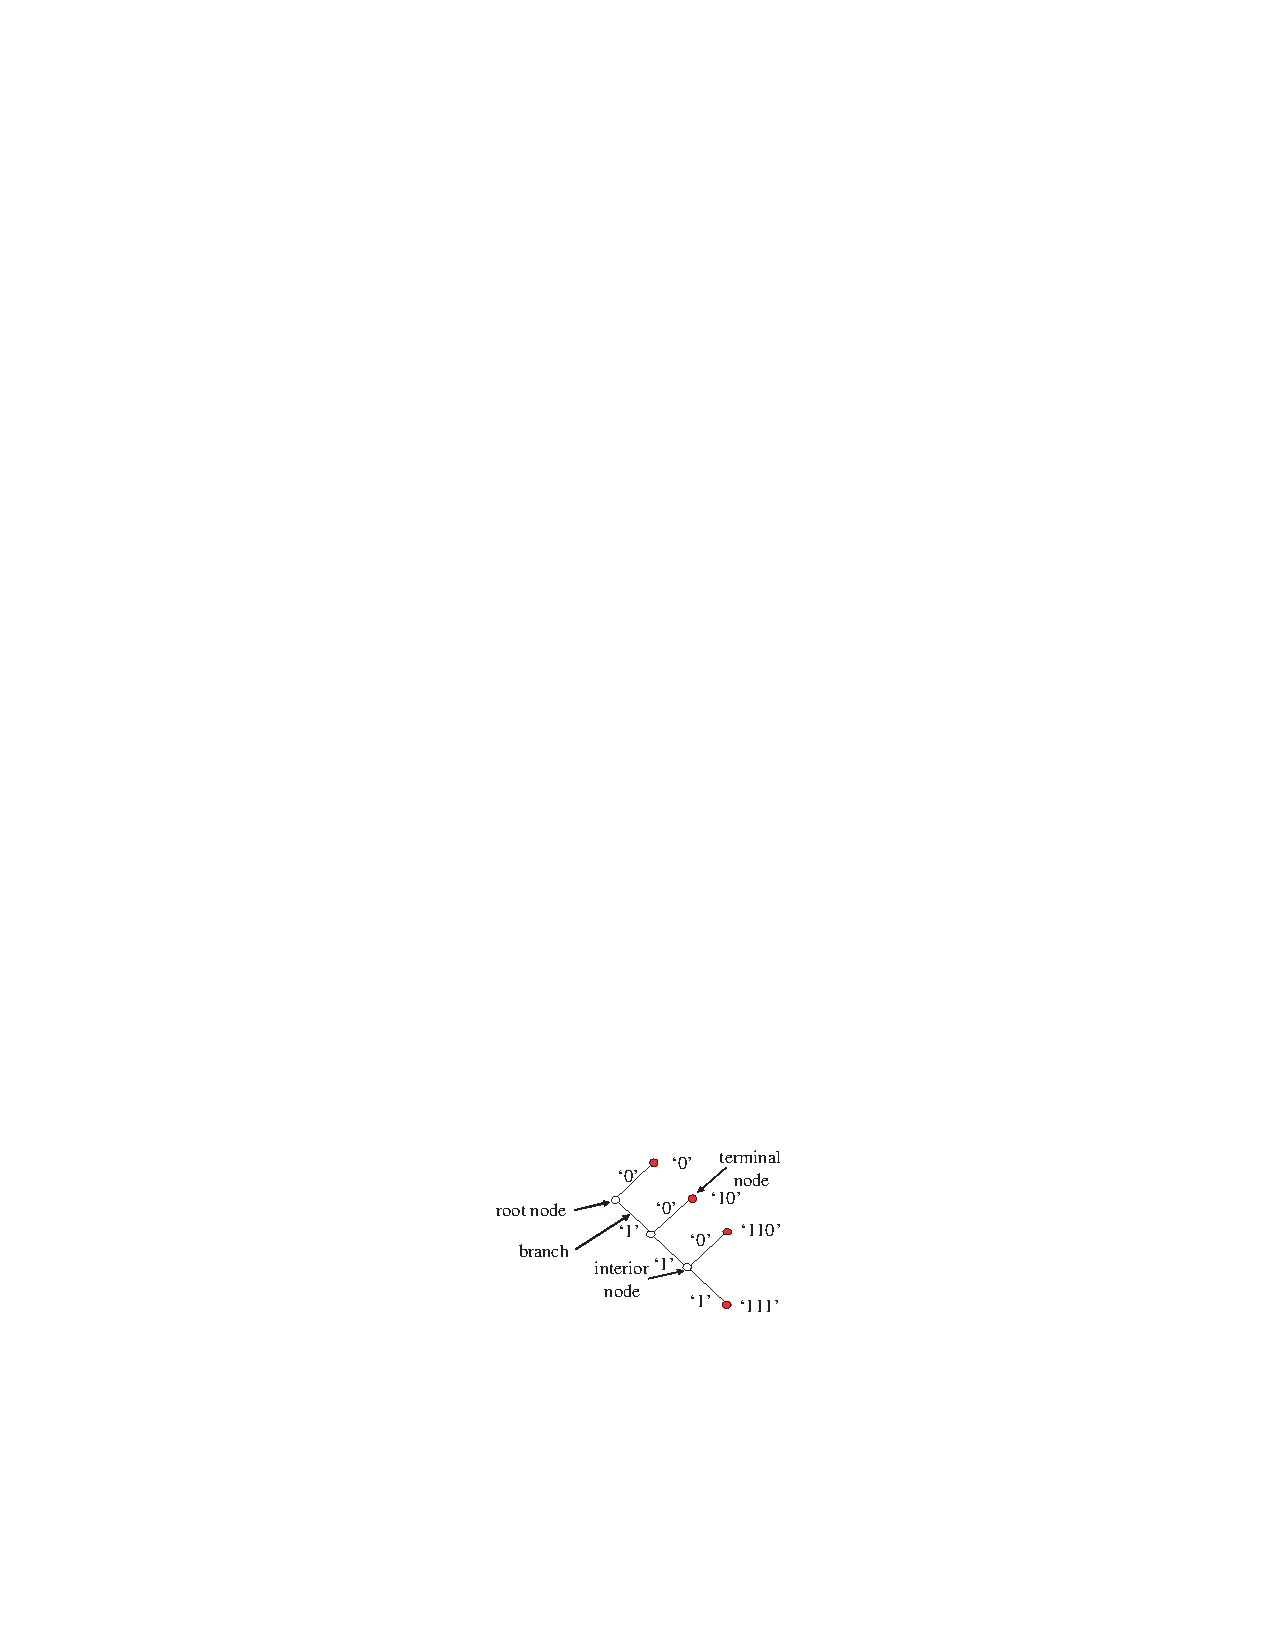
\includegraphics[width=0.5\textwidth]{Figures/PrefixCode}
\caption{Arbre binaire d'un code de $4$ symboles,
qui satisfait la condition de pr\'efixe. }
\label{prefixe6}
\end{figure}

Un code qui satisfait la condition de pr\'efixe peut \^etre
associ\'e \`a un arbre binaire, dont les $K$ feuilles correspondent
aux symboles $\{a_k \}_\UkK$.
Cette repr\'esentation est utile pour construire le code
qui minimise le nombre de bits moyen $R$.
Les branches de gauche et de droite de l'arbre binaire sont
respectivement cod\'ees par 0 et 1.
La figure \ref{prefixe6} montre un exemple pour un code
de $4$ symboles.
Le mot binaire $w_k$ associ\'e au symbole $a_k$
est la succession de $0$ et de $1$ correspondant aux branches
de gauche et de droite, le long du chemin de la racine de
l'arbre \`a la feuille correspondant \`a $a_k$.
Le code binaire g\'en\'er\'e par un tel arbre satisfait toujours
la condition de pr\'efixe. En effet, $w_m$ est
un pr\'efixe de $w_k$ si et seulement si
$a_m$ est un anc\^etre de $a_k$ dans l'arbre binaire.
Ceci n'est pas possible puisque les deux symboles correspondent
\`a des feuilles de l'arbre.
Inversement, tout code pr\'efixe peut \^etre repr\'esent\'e par un tel
arbre binaire.
La longueur $l_k$ du mot binaire
$w_k$ est la profondeur de la feuille $a_k$ dans l'arbre binaire.
L'optimisation d'un code de pr\'efixe est donc \'equivalente \`a
la construction d'un arbre binaire optimal qui distribue
les profondeur des feuilles de fa\c con \`a minimiser
(\ref{bit-rate}).

\subsection{Entropie de Shannon}
Le th\'eor\`eme de Shannon prouve que le nombre moyen de bit $R$
par symbole est plus grand que l'entropie.

\begin{theorem} [Shannon]
\label{shan-th}
On suppose que les symboles
$\{a_k\}_{1 \leq k \leq K}$ apparaissent avec la distribution
de probabilit\'e $\{p(a_k)\}_\UkK$.
Le nombre moyen $R$ de bit d'un code ayant la propri\'et\'e du
pr\'efixe satisfait
\begin{equation}
\label{shan1}
R \geq H = - \sum_{k=1}^K p(a_k) \log_2 p(a_k) .
\end{equation}
Il existe un code ayant la propri\'et\'e du pr\'efixe tel que
\begin{equation}
\label{shan2}
R \leq H + 1.
\end{equation}
\end{theorem}
\begin{proof}
Le th\'eor\`eme de Shannon se d\'emontre \`a partir de
l'in\'egalit\'e de Kraft.

\begin{lemma} [In\'egalit\'e de Kraft]
Tout code ayant la propri\'et\'e du pr\'efixe satisfait
\begin{equation}
\label{kraft}
\sum_{k=1}^K 2^{-l_k} \leq 1 .
\end{equation}
Inversement, si
$\{ l_k \}_\UkK$ sont des entiers positifs tels que
l'in\'egalit\'e (\ref{kraft}) est satisfaite alors il existe
un code de mots binaires $\{w_k \}_\UkK$ de longueurs
$\{ l_k \}_\UkK$ et qui satisfait la condition de pr\'efixe.
\end{lemma}

Pour d\'emontrer (\ref{kraft}) on associe un arbre binaire
au code consid\'er\'e. Chaque $l_k$ correspond \`a un noeud
de l'arbre \`a une profondeur $l_k$ qui d\'epend du mot
binaire $w_k$. Soit
\begin{equation}
\label{mmax}
m = \max \{l_1, l_2, \dots , l_K\} .
\end{equation}
On consid\'ere l'arbre binaire complet dont toutes les
feuilles sont \`a la profondeur $m$.
On note $T_k$ le sous-arbre issu du noeud correspondant au
mot binaire $w_k$. Ce sous arbre a une profondeur ${m - l_k}$
et contient donc $2^{m - l_k}$ noeud au niveau $m$.
Comme il y a $2^m$ noeud \`a la profondeur $m$ de l'arbre binaire
complet et que
la propri\'et\'e du pr\'efixe implique
que tous les sous arbres $T_1 , \dots , T_K$ sont distincts, on
d\'eduit que
\[
\sum_{k=1}^K 2^{m-l_k} \leq 2^m ,
\]
d'o\`u (\ref{kraft}).



Inversement, on consid\`ere $\{ l_k \}_\UkK$ satisfaisant
(\ref{kraft}) avec $l_1 \leq l_2 \leq \dots \leq l_K$ et
$m = \max \{l_1, l_2, \dots , l_K\}$.
On d\'efinit les ensembles $N_1$ des $2^{m-l_1}$ premiers
noeud au niveau $m$ sur la gauche de l'arbre, puis $N_2$
l'ensemble des $2^{m-l_2}$ noeuds suivants et ainsi de suite.
Les noeuds des ensembles $N_k$ sont les noeuds terminaux
de sous-arbres $T_k$ qui sont disjoints. On associe
\`a la racine de l'arbre $T_k$ qui est \`a la profondeur
$l_k$ le mot binaire $w_k$. Cela d\'efinit un code
qui satisfait la condition du pr\'efixe o\`u chaque
mot a la longueur $l_k$ voulue.
Cela termine la d\'emonstration du lemme.

Pour d\'emontrer les deux in\'egalit\'es (\ref{shan1}) et
(\ref{shan2}) du
th\'eor\`eme, on consid\`ere la minimisation de
\[
R = \sum_{k=1}^K p(a_k) \,l_k
\]
sous la contrainte de Kraft
\[
\sum_{k=1}^K 2^{-l_k} \leq 1 .
\]
Dans un premier temps, nous
supposons que $l_k$ peut \^etre un r\'eel quelconque.
Le minimum se calcule en utilisant un multiplicateur de
Lagrange $\lambda$ et en minimisant
\[
J = \sum_{k=1}^K p(a_k) l_k + \lambda \sum_{k=1}^K 2^{-l_k} .
\]
L'annulation de la d\'erivee par rapport \`a $l_k$ donne
\[
\frac {\partial J} {\partial l_k} = p(a_k) - \lambda \,2^{-l_k}\,
\log_{\exp} 2  = 0 .
\]
Le minimum est obtenu pour $\sum_{k=1}^K 2^{-l_k} = 1$
et comme $\sum_{k=1}^K p(a_k) = 1$ on obtient
$\lambda = 1/\log_{\exp} 2$. La longueur optimale minimisant
$R$ est donc
\[
l_k = -\log_2 p(a_k) ,
\]
et
\[
R =
\sum_{k=1}^K p(a_k)\, l_k = - \sum_{k=1}^K p(a_k) \log_2 p(a_k) = H .
\]

Pour garantir que $l_k$ est entier, on choisit
\[
l_k = \lceil - \log_2 p(a_k) \rceil
\]
o\`u $\lceil x \rceil$ est la plus petite valeur enti\`ere
sup\'erieure \`a $x$.
Cela correspond au code de Shannon.
Comme $l_k \geq - \log_2 p(a_k)$, l'in\'egalit\'e
de Kraft est satisfaite puisque
\[
\sum_{k=1}^K 2^{-l_k} \leq \sum_{k=1}^K 2^{\log_2 p(a_k)} = 1 .
\]
Il existe donc un code pr\'efixe dont les mots de code
ont une longueur $l_k$. Pour ce code
\[
\sum_{k=1}^K p(a_k) l_k \leq
\sum_{k=1}^K p(a_k) (-\log_2 p(a_k) + 1) = H + 1 .
\]
\end{proof}

\subsection{Codage par blocs}
L'ajout de 1 bit dans l'in\'egalit\'e (\ref{shan2})
vient du fait que $-\log_2 p_i$ n'est pas n\'ecessairement
un entier alors que la longueur d'un mot binaire doit
\^etre un entier. On peut construire des codes tels que
$R$ est plus proche de $H$ en r\'epartissant ce bit
suppl\'ementaire sur un bloc de $n$ \'el\'ements.
Au lieu de faire un codage instantan\'e, symbole par symbole,
on code d'un coup le bloc de symboles
$\vec X = X_1 , \,\dots\,,X_n$, qui peut \^etre consid\'er\'e
comme une variable al\'eatoire \`a valeurs dans
l'alphabet $A^n$ de taille $K^n$.
A tout bloc de symboles $\vec a \in A^n$ on associe un
mot binaire de longuer $l(\vec a)$. Le nombre de bits
$R$ par symbole pour un tel code par bloc est
\[
R = \frac 1 n \sum_{\vec a \in A^n} p(\vec a) \, l(\vec a) .
\]


\begin{proposition}
\label{shan-prop}
Le nombre moyen $R$ de bit d'un code
par bloc de taille $n$ ayant la propri\'et\'e du
pr\'efixe satisfait
\begin{equation}
\label{shan12}
R \geq H = - \sum_{k=1}^K p(a_k) \log_2 p(a_k) .
\end{equation}
Il existe un code par blocs de taille
$n$ ayant la propri\'et\'e du pr\'efixe tel que
\begin{equation}
\label{shan22}
R \leq H + \frac 1 n.
\end{equation}
\end{proposition}
\begin{proof}
L'entropie associ\'ee \`a $\vec X$ est
\[
\vec H = \sum_{\vec x \in A^n} p(\vec x) \, \log_2 p(\vec x) .
\]
Comme les variables al\'eatoires $X_i$ sont ind\'ependantes
\[
p(\vec x) = p(x_1, \dots , x_n) = \prod_{i=1}^n p(x_i)~.
\]
On d\'emontre par r\'ecurrence sur $n$ que
$\vec H = n H$. Soit $\vec R$ le nombre de bits moyen
pour coder les $n$ symboles $\vec X$. Le th\'eor\`eme
de Shannon \ref{shan-th} montre que $\vec R \geq \vec H$
et qu'il existe un code par bloc tel que
$\vec R \leq \vec H + 1$. On d\'eduit donc
(\ref{shan12},\ref{shan22}) pour $R = \frac{\vec R} n$, qui
est le nombre de bits moyen par symbole.
\end{proof}

Ce th\'eor\`eme d\'emontre que des codes par blocs
utilisent un nombre moyen de bits par symbole qui tendent
vers l'entropie lorsque la taille du bloc augmente.

\subsection{Code de Huffman}
L'algorithme de Huffman est un algorithme de programmation dynamique
qui construit de bas en haut un arbre correspondant \`a un
code pr\'efixe et qui
minimise
\begin{equation}
\label{Rmoyen}
R = \sum_{k=1}^K p(a_k) \, l_k .
\end{equation}
Nous ordonnons
$\{a_k \}_\UkK$ pour que $p(a_k) \leq p(a_{k+1})$.
Pour minimiser (\ref{Rmoyen})
les symboles de plus petites probabilit\'es doivent \^etre
associ\'es aux mot binaires $w_k$ de longueur maximale, ce qui
correspond \`a un noeud au bas de l'arbre.
Nous commen\c cons donc par repr\'esenter les deux symboles de plus
petite probabilit\'e
$a_1$ et $a_2$ comme les enfants d'un noeud commun.
Ce noeud peut \^etre interpr\'et\'e comme un symbole
$a_{1,2}$ correspondant \`a ``$a_1$ ou $a_2$'' et
dont la probabilit\'e est
$p(a_1) + p(a_2)$. La proposition suivante prouve que
l'on peut it\'erer ce regroupement \'el\'ementaire et construire un
code optimal.

\begin{proposition}
On consid\`ere $K$ symboles avec leurs probabilit\'es
ordonn\'ees en ordre croissant: $p(a_k) \leq p(a_{k+1})$.
On regroupe les deux symboles $a_1$ et $a_2$ de probabilit\'e
minimum en un seul symbole $a_{1,2}$ de probabilit\'e
\[
p(a_{1,2}) = p(a_1) + p(a_2) .
\]
Un arbre correspondant \`a un code pr\'efixe optimal pour
les $K$ symboles se construit \`a partir
d'un arbre de code pr\'efixe optimal pour les $K-1$ symboles
$\{a_{1,2}\} \cup \{ a_k \}_{3 \leq k \leq K}$,
en divisant la feuille de
$a_{1,2}$ en deux noeuds correspondant \`a $a_1$ et $a_2$.
\end{proposition}

La d\'emonstration de cette proposition se trouve dans
\cite{bremaud-proba}.

Cette proposition r\'eduit la construction d'un code optimal de
$K$ symboles \`a la construction
d'un code optimal pour les $K-1$ symboles.
Le code de Huffman it\`ere $K-1$ fois
ce regroupement et fait progressivement pousser l'arbre
d'un code de pr\'efixe optimal depuis le bas jusqu'en haut.
Le Th\'eor\`eme \ref{shan-th} de Shannon prouve que
\begin{equation}
\label{entropy-bound}
H \leq R  \leq H + 1 .
\end{equation}
\\
\\
\subsection{Exemple}
Les probabilit\'es des $\{a_k\}_{1 \leq k \leq 6}$ sont
\begin{equation}
\label{proba-code}
\{p(a_k)\}_{1 \leq k \leq 6} = \{0.05~,~0.1~,~0.1~,~0.15~,~0.2~,~0.4\}.
\end{equation}

La figure \ref{arbre-binaire}
donne l'arbre binaire construit avec l'algorithme
de Huffman.
Les symboles $a_1$ et $a_2$ sont regroup\'es
en un symbole $a_{1,2}$
de probabilit\'e $p(a_{1,2}) = p(a_1)+p(a_2)= 0.15$. A l'it\'eration suivante,
les symboles de plus basse probabilit\'e sont
$p(a_3) = 0.1$ et $p(a_{1,2}) = 0.15$. On regroupe donc
$a_{1,2}$ et $a_3$ en un symbole $a_{1,2,3}$ dont la probabilit\'e
est $0.25$. Les deux symboles de probabilit\'es les plus faibles sont
alors $a_4$ et
$a_5$ qui sont regroup\'es en $a_{4,5}$
de probabilit\'e $0.35$. On regroupe ensuite $a_{4,5}$ et
$a_{1,2,3}$ pour obtenir un symbole $a_{1,2,3,4,5}$ de probabilit\'e
$0.6$ qui est finalement regroup\'e avec $a_6$, ce qui finit
le code, comme l'illustre
l'arbre de la figure \ref{arbre-binaire}.
Le nombre moyen de bits obtenu par ce code est
$R= 2.35$ alors que l'entropie est $H = 2.28$.

\begin{figure}[bhtp]
\centerline{
        \epsfxsize=6cm
	\leavevmode\epsfbox{NewFig/fig3.eps}}
\caption {Arbre correspondant au code de Huffman pour une
source dont les probabilit\'es sont donn\'ees par
(\protect \ref{proba-code}) \protect \cite{vetterli}.}
\label{arbre-binaire}
\end{figure}
\\
\\
\noindent
\subsection{Sensibilit\'e au bruit}
Un code de Huffman est plus compact qu'un code de taille fixe
$\log_2 K$ mais est aussi plus sensible au bruit.
Pour un code de taille constante, une erreur
de transmission d'un bit modifie
seulement la valeur d'un symbole.
Au contraire, une erreur d'un bit
dans un code de taille variable peut modifier toute la suite
des symboles.
Lors de transmissions bruit\'ees, de telles erreurs peuvent se
produire. Il est alors n\'ecessaire d'utiliser un code correcteur
qui introduit une l\'eg\`ere redondance de facon \`a identifier les
erreurs.

\section{Quantification scalaire}
\label{scalar-quant-sec}

Si une variable al\'eatoire $X$
prend des valeurs r\'eelles quelconques, on ne peut pas
obtenir un code exact de taille finie.
Il est alors n\'ecessaire d'approximer $X$ par
$\tilde X$ qui prend ses valeurs dans un alphabet fini, et
l'erreur r\'esultante est
\[
D = E \{|X - \tilde X|^2\} .
\]
Un quantificateur scalaire d\'ecompose l'axe r\'eel en
$K$ intervalles $\{[y_{k-1} , y_k ]\}_{1 \leq k \leq K}$
de tailles variables, avec $y_0 = -\infty$ et $y_K = +\infty$.
Le quantificateur associe \`a tout
$x \in [y_{k-1} , y_k]$ une valeur
$Q(x) =a_k$.
Si les $K$ niveaux de quantification $\{a_k\}_{\UkK}$
sont fix\'es a priori,
pour minimiser $|x - Q(x)| = |x - a_k|$,
il faut que la quantification
associe \`a $x$ son niveau de quantification $a_k$ le plus
proche. On doit alors choisir des intervalles de quantification
qui satisfont
\begin{equation}
\label{opt-interv}
y_k = \frac {a_k + a_{k+1}} 2
\end{equation}
\\
\\
\subsection{Quantification haute r\'esolution}
Soit $p(x)$ la densit\'e de probabilit\'e de $X$.
On note $\tilde X = Q (X)$ la variable quantifi\'ee.
L'erreur quadratique moyenne est
\begin{equation}
\label{quantize-error}
D = E\{(X- \tilde X)^2\} =
\int_{-\infty}^{+\infty} |x - Q(x)|^2 p(x) dx .
\end{equation}

On dit que le quantificateur a une haute
r\'esolution si
$p(x)$ peut \^etre approxim\'e par une constante sur tout intervalle
de quantification $[{y_{k-1}},{y_{k}}]$.
La taille de ces intervalles est $\Delta_k = y_k - y_{k-1}$.
L'hypoth\`ese de haute r\'esolution implique que
\begin{equation}
\label{high-resol-quant}
p(x) = \frac {p_k} {\Delta_k} ~~\mbox{pour $x \in [y_{k-1},{y_{k}}]$},
\end{equation}
avec
\[
p_k = \PP \{X \in [{y_{k-1}},y_{k}] \} = \PP \{ \tilde X = a_k \} .
\]
La proposition suivant calcule l'erreur $D$ sous cette hypoth\`ese.

\begin{proposition}
Pour un quantificateur de haute r\'esolution sur des intervalles
$[{y_{k-1}},{y_{k}}]$, l'erreur $D$
minimum obtenue en optimisant la position des niveaux
$\{ a_k \}_{0 \leq k \leq K}$ est
\begin{equation}
\label{quadr-error}
D = \frac 1 {12} \sum_{k=1}^{K} {p_k} \, {\Delta_k ^2} .
\end{equation}
\end{proposition}
\begin{proof}
Comme $Q(x) = a_k$ si
$x \in [y_{k-1},y_k)$, on peut re\'ecrire (\ref{quantize-error})
\[
D = \sum_{k=1}^{K} \int_{y_{k-1}}^{y_{k}} (x - a_k)^2 p(x) dx .
\]
En rempla\c{c}ant $p(x)$ par son expression
(\ref{high-resol-quant}) on a
\begin{equation}
D =
\sum_{k=1}^{K} \frac {p_k} {\Delta_k}
\int_{y_{k-1}}^{y_{k}} (x - a_k)^2  dx.
\end{equation}
Cette erreur est minimum
pour $a_k = \half (y_{k}+{y_{k-1}})$, et l'int\'egration donne
(\ref{quadr-error}).
\end{proof}

\subsection{Quantification uniforme}
Le quantificateur uniforme est un cas particulier important o\`u
tous les intervalles de quantification sont de m\^eme taille
\[
y_{k} - y_{k-1} = \Delta ~~~\mbox{pour $1 \leq k \leq K$} .
\]
L'erreur quadratique moyenne (\ref{quadr-error})
devient
\begin{equation}
\label{unifoquantiz}
D = \frac {\Delta^2} {12} \sum_{k=1}^{K} {p_k}
= \frac {\Delta^2} {12} .
\end{equation}
Elle est ind\'ependante de la distribution de probabilit\'e
$p(x)$ de la source.
\\
\\
\subsection{Quantification optimale}
On veut optimiser
le quantificateur pour minimiser le nombre de bits
n\'ecessaires pour coder les valeurs quantifi\'ees
$\tilde X$, \'etant donn\'ee une distortion $D$ admissible.
Le th\'eor\`eme de
Shannon \ref{shan-th} prouve que la valeur moyenne minimum de bits
n\'ecessaire pour coder $\tilde X$ est sup\'erieure \`a l'entropie $H$
de la variable al\'eatoire $\tilde X$.
Comme le
code de Huffman donne un r\'esultat proche de cette entropie,
il nous faut minimiser l'entropie $H$ pour $D$ fixe.

La source quantifi\'ee $\tilde X$ prend $K$ valeurs diff\'erentes
$\{a_k\}_{1 \leq k \leq K}$ avec probabilit\'es
$\{p_k\}_{1 \leq k \leq K}$.
L'entropie du signal quantifi\'e est donc
\[
H = - \sum_{k=1}^K p_k\, \log_2 p_k .
\]
On d\'efinit l'entropie diff\'erentielle de la variable al\'eatoire
$X$ \`a valeurs r\'eelles
\begin{equation}
\label{entropie-dffD}
H_d = - \int_{-\infty}^{+\infty} p(x) \log_2 p(x) dx .
\end{equation}
Le th\'eor\`eme suivant montre que pour un quantificateur de haute
r\'esolution produisant une erreur $D$,
l'entropie est minimum lorsque le quantificateur est
uniforme.

\begin{theorem}
\label{quanti-theo}
L'entropie de
tout quantificateur de haute r\'esolution satisfait
\begin{equation}
\label{lower-quantX}
H \geq H_d - \frac 1 2 \log_2 (12 D) .
\end{equation}
Le minimum est atteint si et seulement si $Q$ est un
quantificateur uniforme.
\end{theorem}
\begin{proof}
Pour un quantificateur de haute r\'esolution
$p(x)$ est approximativement constant sur $[y_{k-1},y_k]$
et donc
\[
p_k = \int_{y_{k-1}}^{y_k} p(x)\,dx = p_k \Delta_k
\]
avec $\Delta_k = y_k - y_{k-1}$.
Donc
\begin{eqnarray*}
H & = & - \sum_{k=1}^K p_k \log_2 (p(a_k)\, \Delta_k )\\
& = &- \sum_{k=1}^K \int_{y_{k-1}}^{y_k} p(x) \log_2 p(a_k)\, dx
- \sum_{k=1}^K p_k \log_2 \Delta_k \\
& = & H_d - \frac 1 2 \sum_{k=1}^K p_k \log_2 \Delta_k^2 ,
\end{eqnarray*}
car $p(x) = p(a_k)$ pour $x \in [y_{k-1},y_k]$.
Pour toute fonction concave $\phi (x)$, l'in\'egalit\'e de Jensen
montre que pour tout $\sum_{k=1}^K p_k = 1$
et $\{a_k \}_\UkK$ alors
\begin{equation}
\label{jensen}
\sum_{k=1}^N p_k \phi ( a_k) \leq \phi(\sum_{k=1}^N  p_k a_k) .
\end{equation}
Si $\phi (x)$ est strictement concave, l'in\'egalit\'e devient une \'egalit\'e
si et seulement si tous les $a_k$ sont \'egaux lorsque
$p_k \neq 0$. Comme $\log_2(x)$ est strictement concave,
(\ref{quadr-error}) montre que
\[
 \frac 1 2 \sum_{k=1}^N p_k \log_2 \Delta_k^2 \leq
 \frac 1 2 \log_2 \sum_{k=1}^N p_k \Delta_k^2 =
 \frac 1 2 \log_2 (12 D ) .
\]
On en d\'eduit donc que
\[
H \geq H_d - \frac 1 2 \log_2 (12 D ).
\]
Cette in\'egalit\'e devient une \'egalit\'e si et seulement si tous les
$\Delta_k$ sont \'egaux, ce qui correspond \`a un quantificateur
uniforme.
\end{proof}
Ce th\'eor\`eme montre que pour un quantificateur haute r\'esolution
le nombre minimum de bits
$R = H$ est obtenu pour un quantificateur uniforme et
\begin{equation}
\label{bit-rate-uniform}
R = H_d -  \frac 1 2 \log_2 (12 D ).
\end{equation}
La distortion en fonction du nombre de bits est donc
\[
D(R) = \frac 1 {12}\, 2^{2 H_d} \,2^{-2R} .
\]
